% !TeX TXS-program:compile = txs:///xelatex
\documentclass[crop,tikz]{standalone}

\usepackage{etoolbox}
\usepackage{fontspec}
\setmainfont{Fira Sans}

\usetikzlibrary{shapes.geometric}
\usetikzlibrary{calc}
\usetikzlibrary{shadings}
\usetikzlibrary{fadings}
\usetikzlibrary{decorations.markings}
\usetikzlibrary{positioning}

\newcommand*{\arrowpos}{0.8*\pgfdecoratedpathlength-3pt}
\newcommand*{\arrowposs}{0.8*\pgfdecoratedpathlength+5pt}

\newcommand{\drawMirror}[2]{
	\begin{scope}[shift={(#1)},rotate=#2]
		%Now just draw a mirror
		\fill[fill=lightgray] (-0.75,0) rectangle(0.75,0.075);

		\draw (-0.75,0) -- (0.75,0);

		\foreach \x in {-0.75,-0.65,...,0.75}
			%Draw a little diagonal dash
			\draw[cap=round] (\x,0) -- (\x+0.1,0.075);
	\end{scope}
}

\newcommand{\drawHalfMirror}[2]{
	\begin{scope}[shift={(#1)},rotate=#2]
		%Now just draw a mirror
		\fill[fill=lightgray] (-0.75,0) rectangle(0.75,0.075);

		\draw (-0.75,0) -- (0.75,0);
	\end{scope}
}

\newcommand{\drawBeam}[2]{
	\draw[cap=butt, Blue] (#1) -- (#2);
	\draw[cap=butt,Red] (#1) -- (#2);
	\draw[cap=butt,Purple] (#1) -- (#2);
}

\begin{document}
	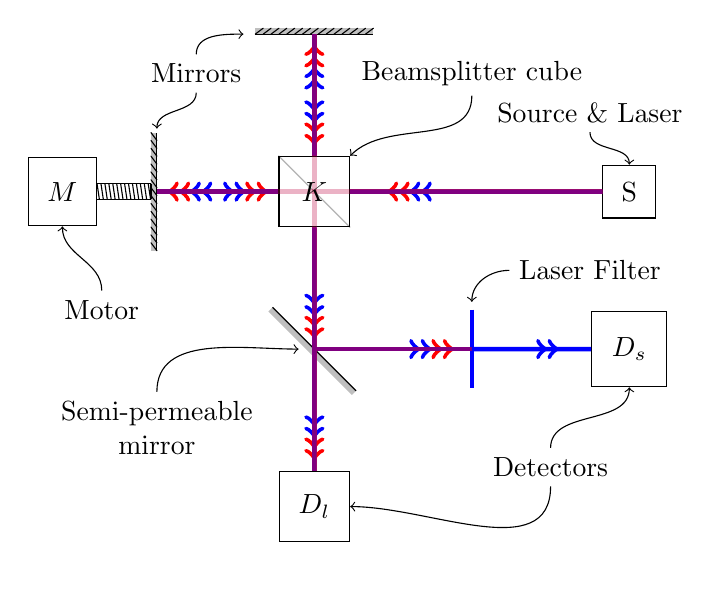
\begin{tikzpicture}
		\tikzstyle{Mirror} = [ultra thick, black]
		\tikzstyle{Blue} = [ultra thick, blue, decoration={markings,
			mark=at position \arrowpos with \arrow{>>}}, postaction=decorate]
		\tikzstyle{Red} = [ultra thick, red, decoration={markings,
			mark=at position \arrowposs with \arrow{>>}}, postaction=decorate]
		\tikzstyle{Purple} = [violet, ultra thick]

		%Draw cube
		\node[regular polygon, regular polygon sides = 4, draw=black, fill=white, text width=0.4cm](K) at (5,3.65){};
		\draw[opacity=0.3] (K.north west) -- (K.south east);

		%Draw mirrors
		\coordinate (M1) at ($(K) + (0,2)$);
		%\draw[Mirror] ($(M1) + (0.75,0)$) --($(M1) - (0.75,0)$);
		\drawMirror{M1}{0}
		\coordinate (M2) at ($(K) - (2,0)$);
		\drawMirror{M2}{90}

		\coordinate (M3) at ($(K) - (0,2)$);
		\drawHalfMirror{M3}{135}

		\node[fill=white, draw=black, regular polygon, regular polygon sides=4] (S) at ($(K) + (4,0)$){S};
		\coordinate (F) at ($(M3) + (2,0)$);
		\node[fill=white, draw=black, regular polygon, regular polygon sides=4] (S1) at ($(F) + (2,0)$){$D_s$};
		\node[fill=white, draw=black, regular polygon, regular polygon sides=4] (S2) at ($(M3) - (0,2)$){$D_l$};


		%Draw beams
		\drawBeam{K}{M1}
		\drawBeam{M1}{K}
		\drawBeam{K}{M2}
		\drawBeam{M2}{K}
		\drawBeam{S}{K}
		\drawBeam{K}{M3}

		\begin{scope}[opacity=0.3]
			\draw[ultra thick, purple] (K.east) -- (K.west);
			\draw[ultra thick, purple] (K.north) -- (K.south);
		\end{scope}

		\node(KLabel) at (5,3.65){$K$};

		\draw[blue, ultra thick] ($(F) + (0,0.5)$) -- ($(F) - (0,0.5)$);
		\drawBeam{M3}{F}
		\drawBeam{M3}{S2}

		\draw[Blue] (F) -- (S1);


		%Draw the Mirror movement mechanism
		\draw ($(M2) + (-0.075,0.1)$) -- ($(M2) + (-1,0.1)$) -- ($(M2) + (-1,-0.1)$) -- ($(M2) + (-0.075,-0.1)$);
		\draw ($(M2) + (-1,0.1)$) -- ($(M2) + (-1,-0.1)$);
		\draw ($(M2) + (-0.075,0.1)$) -- ($(M2) + (-0.075,-0.1)$);

		\foreach \x in {-1,-0.95,...,-0.1}{
			\draw ($(M2) + (\x+0.04,0.1)$) -- ($(M2) + (\x+0.07,-0.1)$);
		}

		\node[fill=white,draw=black,regular polygon,regular polygon sides=4](M) at ($(M2) + (-1.2,0)$){$M$};

		%Labels
		\node(Mirrors) at ($(K) + (-1.5,1.5)$){Mirrors};
		\draw[->] (Mirrors.north) to[in=180,out=90] ($(M1)+(-0.9,0)$);
		\draw[->] (Mirrors.south) to[in=90,out=-90] ($(M2) + (0,0.8)$);

		\node(Detectors) at ($(S1) + (-1,-1.5)$){Detectors};
		\draw[->] (Detectors.north) to[in=-90,out=90] (S1.south);
		\draw[->] (Detectors.south) to[in=0,out=-90] (S2.east);

		\node(Motor) at ($(M) + (0.5,-1.5)$){Motor};
		\draw[->] (Motor.north) to[out=90,in=-90] (M.south);

		\node[align=center](SemMir) at ($(M3) + (-2,-1)$){Semi-permeable \\mirror};
		\draw[->] (SemMir.north) to[out=90,in=180] ($(M3.west) + (-0.2,0)$);

		\node (Filter) at ($(F) + (1.5,1)$){Laser Filter};
		\draw[->] (Filter.west) to[out=180,in=90] ($(F) + (0,0.6)$);

		\node (Cube) at ($(K) + (2,1.5)$){Beamsplitter cube};
		\draw[->] (Cube.south) to[out=-90,in=45] (K.north east);

		\node (Source) at ($(S) + (-0.5,1)$){Source \& Laser};
		\draw[->] (Source.south) to [out=-90,in=90] (S.north);
	\end{tikzpicture}
\end{document}
